\boxde
\BTTN
\Opensolutionfile{ans}[ans/2D1-4-DEON-1]
\begin{ex}%[2D1B4-1]
    Cho hàm số $y=f(x)$ có bảng biến thiên như hình bên. Đồ thị hàm số đã cho có tiệm cận ngang là đường thẳng
    \begin{center}
        
\begin{tikzpicture}[scale=0.8, font=\footnotesize, line join=round, line
            cap=round, >=stealth]
            \tkzTabInit[espcl=2.5,lgt=1,nocadre=false]
            {$x$/0.7,$f(x)$/2.1}
            {$-\infty$,$0$,$1$,$2$,$+\infty$}
            \tkzTabVar{-/$-\infty$,+/$2$,-D+/$-\infty$/$+\infty$,-/$4$,+/$6$}
        \end{tikzpicture}
    \end{center}
    \choice
    {$y=2$}
    {$y=1$}
    {\True $y=6$}
    {$y=4$}
    \loigiai{Dựa vào bảng biến thiên ta thấy đồ thị hàm có tiệm cận ngang $y=6$.
    }
\end{ex}
%56
\begin{ex}%[2D1B4-1]
    Cho hàm số $y=f(x)$ có bảng biến thiên như hình bên. Tổng số tiệm cận đứng và tiệm cận ngang của đồ thị hàm số đã cho là
    \begin{center}
        
\begin{tikzpicture}[scale=0.8]
            \tkzTabInit[nocadre=false,lgt=1.5,espcl=3,deltacl=0.6]
            {$x$ /0.6,$y’$ /0.6,$y$ /2}
            {$-\infty$ , $1$, $+\infty$}
            \tkzTabLine{,+,d,+,}
            \tkzTabVar{-/$2$,+D-/$+\infty$/$3$,+/$5$}
        \end{tikzpicture}
    \end{center}
    \choice
    {$1$}
    {\True $3$}
    {$2$}
    {$4$}
    \loigiai{Dựa vào bảng biến thiên ta thấy đồ thị hàm số có tiệm cận đứng $x=1$ và tiệm cận ngang $y=2$ và $y=5$.}
\end{ex}
\begin{ex}%[2D1B4-1]
    Cho hàm số $y=f(x)$ có bảng biến thiên như hình bên. Tổng số tiệm cận đứng và tiệm cận ngang của đồ thị hàm số đã cho là
    \begin{center}
        
\begin{tikzpicture}[scale=0.8]
            \tkzTabInit[nocadre=false,lgt=1.5,espcl=3,deltacl=0.6]
            {$x$ /0.6,$y’$ /0.6,$y$ /2}
            {$-\infty$ ,$0$, $1$, $+\infty$}
            \tkzTabLine{,+,0,-,d,-,}
            \tkzTabVar{-/$4$,+/$2$,-D+/$-1$/$+\infty$,-/$-3$}
        \end{tikzpicture}
    \end{center}
    \choice
    {$1$}
    {\True $3$}
    {$2$}
    {$4$}
    \loigiai{
        Dựa vào bảng biến thiên ta thấy đồ thị hàm số có tiệm cận đứng $x=1$, tiệm cận ngang $y=4$ và $y=-3$.
    }
\end{ex}
%61
\begin{ex}%[2D1B4-1]
    Cho hàm số $y=f(x)$ có bảng biến thiên như hình bên. Tổng số tiệm cận đứng và tiệm cận ngang của đồ thị hàm số đã cho là
    \begin{center}
        
\begin{tikzpicture}[scale=0.8]
            \tkzTabInit[nocadre=false,lgt=1.5,espcl=3,deltacl=0.6]
            {$x$ /0.6,$y’$ /0.6,$y$ /2}
            {$-\infty$ ,$0$, $1$, $+\infty$}
            \tkzTabLine{,-,0,+,d,+,}
            \tkzTabVar{+/$5$,-/$-4$,+D-/$+\infty$/$-\infty$,+/$2$}
        \end{tikzpicture}
    \end{center}
    \choice
    {$1$}
    {\True $3$}
    {$2$}
    {$4$}
    \loigiai{Dựa vào bảng biến thiên ta thấy đồ thị hàm số có một tiệm cận đứng $x=1$, hai tiệm cận ngang $y=5$ và $y=2$.}
\end{ex}
\begin{ex}%[2D1B4-1]
    Đồ thị hàm số nào trong các hàm số dưới đây có tiệm cận đứng?
    \choice
    {\True $y=\dfrac{1}{\sqrt{x}}$}
    {$y=\dfrac{1}{x^2+x+1}$}
    {$y=\dfrac{1}{x^4+1}$}
    {$y=\dfrac{1}{x^2+1}$}
    \loigiai{
    }
\end{ex}
\begin{ex}%[2D1K4-1]
    Số tiệm cận đứng của đồ thị hàm số $y=\dfrac{\sqrt{x+4}-2}{x^2+x}$ là
    \choice
    {$3$}
    {$0$}
    {$2$}
    {\True $1$}
    \loigiai{
        Tập xác định hàm số $ \mathscr{D}=[-4;+\infty)\setminus\lbrace -1;0\rbrace
        $.\\
        Ta có $ \lim\limits_{x\to -1^{+}}y=+\infty $, $ \lim\limits_{x\to 0^{+}}y=1
        $ và $ \lim\limits_{x\to 0^{-}}y=1 $.\\
        Suy ra đồ thị hàm số chỉ có $ 1 $ tiệm cận đứng là $ x=-1 $.
    }
\end{ex}
\begin{ex}%[Nguyễn Văn Sang, dự án Tex hoá đề cương trường Marie Curie - Lần 6]%[2D1Y4-1]
    Đường thẳng nào dưới đây là tiệm cận ngang của đồ thị hàm số $y=\dfrac{3+2 x}{x+1}$?
    \choice
    {$y=3$}
    {$x=-1$}
    {\True $y=2$}
    {$x=2$}
    \loigiai{
        Tập xác định $\mathscr{D}=\mathbb{R}\setminus\left\lbrace -1\right\rbrace$.
        \begin{itemize}
            \item $\lim\limits_{x \to \pm\infty} y=\lim\limits_{x \to \pm\infty} \dfrac{3+2 x}{x+1}=2$ suy ra $y=2$ là tiệm cận ngang.
            \item $\heva{& \lim\limits_{x \to -1^+} \dfrac{3+2 x}{x+1}=+\infty \\ & \lim\limits_{x \to -1^-} \dfrac{3+2 x}{x+1}=-\infty}$ suy ra $x=-1$ là tiệm cận đứng.
        \end{itemize}
    }
\end{ex}
%%=====Câu 15
\begin{ex}%[2D1Y4-1]
    Giao điểm của tiệm cận đứng và tiệm cận ngang của đồ thị hàm số $y=\dfrac{3x-2}{1-x}$ là điểm
    \choice
    {$M(1;3)$}
    {$P(-3;1)$}
    {\True $Q(1;-3)$}
    {$N\left(\dfrac{2}{3};3\right)$}
    \loigiai{
        Tiệm cận đứng, tiệm cận ngang của đồ thị hàm số lần lượt là $x=1$ và $y=-3$. Giao điểm của $2$ tiệm cận là $Q(1;-3)$.
    }
\end{ex}
\begin{ex}%[2D1K4-2]%
    Nếu đồ thị hàm số $y=\dfrac{(m+1)x+2}{x-n+1}$ lần lượt nhận trục hoành và trục tung làm đường đường tiệm cận ngang và tiệm cận đứng thì $m+n$ bằng bao nhiêu?
    \choice
    {\True $m+n=0$}
    {$m+n=2$}
    {$m+n=-1$}
    {$m+n=1$}
    \loigiai{
        Theo đề bài, ta có $\heva{&m+1=0\\&n-1=0} \Leftrightarrow \heva{&m=-1\\&n=1.}$\\
        Suy ra $m+n=0$.
    }
\end{ex}
\begin{ex}%[2D1K4-1]
    Cho hàm số $y=f(x)$ có bảng biến thiên như hình bên. Đồ thị hàm số $y=\dfrac{x-2}{f(x)-1}$ có bao nhiêu tiệm cận đứng?
    \begin{center}
        
\begin{tikzpicture}
            \tkzTabInit[espcl=3]{$x$ / 1 , $f’(x)$ / 1, $f(x)$ / 2}
            {$-\infty$, $-1$ , $5$, $+\infty$}%
            \tkzTabLine{,-,0,+,0,-,}%
            \tkzTabVar{+/ $+\infty$, - / $-1$, + / $3$,-/$-2$}%
            \tkzTabVal[draw]{2}{3}{0.4}{$2$}{$1$}
        \end{tikzpicture}
    \end{center}
    \choice
    {$1$}
    {$3$}
    {\True $2$}
    {$4$}
    \loigiai{
        Dựa vào bảng biến thiên suy ra
        $f(x)-1=0 \Leftrightarrow f(x) =1$, phương trình này có $2$ nghiệm phân biệt khác $2$ và một nghiệm $x=2$ nên đồ thị hàm số $y=\dfrac{x-2}{f(x)-1}$ có hai tiệm cận đứng.
    }
\end{ex}
%68
\begin{ex}%[2D1K4-1]
    Cho hàm số $y=f(x)$ có bảng biến thiên như hình bên. Đồ thị hàm số $y=\dfrac{1}{2f(x)+1}$ có bao nhiêu tiệm cận đứng?
    \begin{center}
        
\begin{tikzpicture}[scale=0.8]
            \tkzTabInit[nocadre=false,lgt=1.5,espcl=3,deltacl=0.6]
            {$x$ /0.6,$y’$ /0.6,$y$ /2}
            {$-\infty$ ,$-2$, $2$, $+\infty$}
            \tkzTabLine{,+,0,-,0,+,}
            \tkzTabVar{-/$-\infty$,+/$3$,-/$0$,+/$+\infty$}
        \end{tikzpicture}
    \end{center}
    \choice
    {\True $1$}
    {$3$}
    {$2$}
    {$0$}
    \loigiai{
        Dựa vào bảng biến thiên suy ra
        $2f(x)+1=0 \Leftrightarrow f(x) =-\dfrac{1}{2}$, phương trình này có $1$ nghiệm nên đồ thị hàm số $y=\dfrac{1}{2f(x)+1}$ có một tiệm cận đứng.
    }
\end{ex}
\begin{ex}%[2D1K4-1]
    Cho hàm số $y=f(x)$ có bảng biến thiên như hình bên. Đồ thị hàm số $y=\dfrac{1}{2f(x)-1}$ có bao nhiêu tiệm cận ngang?
    \begin{center}
        
\begin{tikzpicture}[scale=0.8]
            \tkzTabInit[nocadre=false,lgt=1.5,espcl=3,deltacl=0.6]
            {$x$ /0.6,$y’$ /0.6,$y$ /2}
            {$-\infty$, $2$, $+\infty$}
            \tkzTabLine{,-,0,+,}
            \tkzTabVar{+/$1$,-/$-3$,+/$1$}
        \end{tikzpicture}
    \end{center}
    \choice
    {$1$}
    {\True $3$}
    {$2$}
    {$0$}
    \loigiai{
        Dựa vào bảng biến thiên suy ra
        \begin{itemize}
            \item 	$\lim \limits_{x \to \pm \infty} f(x)=1 \Leftrightarrow \lim \limits_{x \to \pm \infty}\dfrac{1}{2f(x)-1} =1$ nên đồ thị hàm số đã cho có tiệm cận ngang là $y=1$.
            \item $2f(x)-1=0 \Leftrightarrow f(x)=\dfrac{1}{2}$, phương trình này có $2$ nghiệm phân biệt nên đồ thị hàm số đã cho có hai tiệm cận đứng.
        \end{itemize}
    }
\end{ex}
%80
\begin{ex}%[2D1K4-1]
    Cho hàm số $y=f(x)$ có bảng biến thiên như hình bên. Đồ thị hàm số $y=\dfrac{1}{f^2(x)+f(x)}$ có bao nhiêu tiệm cận đứng?
    \begin{center}
        
\begin{tikzpicture}[scale=0.8]
            \tkzTabInit[nocadre=false,lgt=1.5,espcl=3,deltacl=0.6]
            {$x$ /0.6,$y’$ /0.6,$y$ /2}
            {$-\infty$ ,$-4$, $6$, $+\infty$}
            \tkzTabLine{,-,0,+,0,-,}
            \tkzTabVar{+/$+\infty$,-/$-2$,+/$5$,-/$-\infty$}
        \end{tikzpicture}
    \end{center}
    \choice
    {$4$}
    {$3$}
    {$2$}
    {\True $6$}
    \loigiai{
        Dựa vào bảng biến thiên suy ra $f^2(x)+f(x)=0 \Leftrightarrow \hoac{&f(x)=0\\&f(x)=-1}$, mỗi phương trình này có $3$ nghiệm phân biệt nên đồ thị hàm số đã cho có $6$ tiệm cận đứng.
    }
\end{ex}
\begin{ex}%[2D1K4-1]
    Cho hàm số $y=f(x)$ có bảng biến thiên như hình bên. Đồ thị hàm số $y=\dfrac{3}{f(x^2)+1}$ có bao nhiêu tiệm cận đứng?
    \begin{center}
        
\begin{tikzpicture}[scale=0.8]
            \tkzTabInit[nocadre=false,lgt=1.5,espcl=3,deltacl=0.6]
            {$x$ /0.6,$y’$ /0.6,$y$ /2}
            {$-\infty$ ,$0$, $2$, $+\infty$}
            \tkzTabLine{,+,d,-,0,+,}
            \tkzTabVar{-/$-\infty$,+/$1$,-/$-2$,+/$+\infty$}
        \end{tikzpicture}
    \end{center}
    \choice
    {\True $4$}
    {$3$}
    {$6$}
    {$0$}
    \loigiai{
        Dựa vào bảng biến thiên suy ra
        $f(x^2)+1=0 \Leftrightarrow f(x^2) =-1$. Kẻ đường thẳng $y=-1$ ta thấy đường thẳng cắt đồ thị hàm số tại 3 điểm phân biệt. Suy ra
        $$\hoac{&x^2=a \; (a<0)\\&x^2=b \; (b \in (0;2)\\&x^2=c \; (c>2)} \Rightarrow \hoac{&x=\pm \sqrt{b}\\&x=\pm \sqrt{c}.}$$
        Do đó đồ thị hàm số $y=\dfrac{2}{f(x^2)+1}$ có $4$ tiệm cận đứng.
    }
\end{ex}
\BTTF
\begin{ex}%[EX-TF-2024, Lê Đạt]%[2D1N4-1]
    Cho hàm số $y=\dfrac{2x-3}{x-1}$. Xét tính đúng sai các khẳng định dưới đây
    \choiceTF
    {\True Đường tiệm cận đứng của đồ thị hàm số là $ x=1 $}
    {Đường tiệm cận đứng của đồ thị hàm số là $ y=2 $}
    {Đường tiệm cận ngang của đồ thị hàm số là $ x=1 $}
    {\True Đường tiệm cận ngang của đồ thj hàm số là $ y=2 $}
    \loigiai{
        Ta có $\lim\limits_{x\to -\infty}y=\lim\limits_{x\to +\infty}y=2$ nên đồ thị hàm số đã cho có tiệm cận ngang là $y=2$.\\
        Ta có $\lim\limits_{x\to 1^+}y=-\infty$ nên đồ thị hàm số đã cho có tiệm cận ngang là $ x=1 $.
        \begin{itemchoice}
            \itemch Đường tiệm cận đứng của đồ thị hàm số là $ x=1 $.
            \itemch Đường tiệm cận đứng của đồ thị hàm số là $ x=1 $.
            \itemch Đường tiệm cận ngang của đồ thj hàm số là $ y=2 $.
            \itemch Đường tiệm cận ngang của đồ thj hàm số là $ y=2 $.
        \end{itemchoice}
    }
\end{ex}
%===== DẠNG 2
\begin{ex}%[EX-TF-2024, Lê Đạt]%[2D1H4-2]
    Cho hàm số $ y=\dfrac{m^2x+1}{x-1} $. Xét tính đúng sai của các khẳng định sau
    \choiceTF
    {\True Đồ thị hàm số luôn có tiệm cận ngang}
    {\True Đồ thị hàm số luôn có tiệm cận đứng}
    {\True Khi $ m=1$ đồ thị hàm số có $ 2 $ đường tiệm cận}
    {Khi $ m=0 $ đồ thị hàm số có $ 1 $ đường tiệm cận}
    \loigiai{
        \begin{itemchoice}
            \itemch $\lim\limits_{x\to -\infty}y=\lim\limits_{x\to +\infty}y=m^2$ suy ra hàm số luôn có tiệm cận ngang.
            \itemch $\lim\limits_{x\to 1^+}y=+\infty$ nên đồ thị hàm số đã cho có tiệm cận ngang là $ x=1 $.
            \itemch Khi $ m=1 $ ta được hàm số $ y=\dfrac{x+1}{x-1} $ suy ra đồ thì hàm số có $ x=1 $ là tiệm cận đứng và $ y=1 $ là tiệm cận ngang nên đồ thị hàm số có $ 2 $ tiệm cận.
            \itemch Khi $ m=0 $ ta được hàm số $ y=\dfrac{1}{x-1} $ suy ra đồ thì hàm số có $ x=1 $ là tiệm cận đứng và $ y=0 $ là tiệm cận ngang nên đồ thị hàm số có $ 2 $ tiệm cận.
        \end{itemchoice}
    }
\end{ex}
%===== DẠNG 3
\begin{ex}%[EX-TF-2024, Lê Đạt]%[2D1N4-3]
    \immini{Cho hàm số $y=f(x)$ có đồ thị như hình bên. Xét tính đúng sai của các khẳng định sau
        \choiceTF
        {$ x=2 $ là đường tiệm cận ngang của đồ thị hàm số}
        {\True $ x=-1 $ là đường tiệm cận đứng của đồ thị hàm số}
        {\True Đồ thị hàm số có hai đường tiệm cận}
        {\True Đồ thị hàm số không có tiệm cận xiên}
    }{
        \begin{tikzpicture}[scale=0.5, font=\footnotesize, line join=round, line cap=round, >=stealth]
            \draw[->](-5,0)--(5,0)node[below]{ $x$};
            \draw[->](0,-4)--(0,5)node[right]{ $y$};
            \draw [fill=black,draw=black] (0,0) circle (1pt)node[above left] { $O$};
            \foreach \x in {-1}\draw[shift={(\x,0)}](0pt,-2pt)--(0pt,2pt) node[below left]{ $\x$};
            \foreach \y in {2}\draw[shift={(0,\y)}](-2pt,0pt)--(2pt,0pt)node[above right]{ $\y$};
            \clip(-5,-4) rectangle (5,5);
            \draw[smooth,samples=100,domain=-5:-1.1] plot(\x,{(2*(\x)-1)/((\x)+1)});
            \draw[smooth,samples=100,domain=-0.9:5] plot(\x,{(2*(\x)-1)/((\x)+1)});
            \draw[dashed](-5,2)--(5,2) (-1,-4)--(-1,5);
        \end{tikzpicture}
    }
    \loigiai{
        \begin{itemchoice}
            \itemch $ y=2 $ là đường tiệm cận ngang của đồ thị hàm số.
            \itemch $ x=-1 $ là đường tiệm cận đứng của đồ thị hàm số.
            \itemch $ x=-1 $ là đường tiệm cận đứng và $ y=2 $ là đường tiệm cận ngang của đồ thị hàm số suy ra đồ thị hàm số có hai đường tiệm cận.
            \itemch Đồ thị hàm số không có tiệm cận xiên.
        \end{itemchoice}
    }
\end{ex}
\BTTL
\begin{ex}%[2D1K4-2]%
    Đường tiệm cận đứng và tiệm cận ngang của đồ thị hàm số $y=\dfrac{mx+1}{2m+1-x}$ cùng với hai trục tọa độ tạo thành một hình chữ nhật có diện tích bằng $3$. Khi đó $m$ bằng
    \shortans{$1$ hay $-\dfrac{3}{2}$}
    % \choice
    % {$1$ hay $\dfrac{3}{2}$}
    % {$-1$ hay $-\dfrac{3}{2}$}
    % {\True $1$ hay $-\dfrac{3}{2}$}
    % {$-1$ hay $3$}
    \loigiai{
        Từ yêu cầu đề bài, suy ra $|-m| \cdot |2m+1|=3 \Leftrightarrow \hoac{&m=1\\&m=-\dfrac{3}{2}.}$
    }
\end{ex}
\begin{ex}%[2D1K4-2]%
    Tìm tất cả các giá trị thực $m$ sao cho đồ thị hàm số $y=\dfrac{5x-3}{x^2-2mx+1}$ không có tiệm cận đứng.
    \shortans{$-1<m<1$}
    % \choice
    % {\True $-1<m<1$}
    % {$m=1$}
    % {$m=-1$}
    % {$m <-1$ hoặc $m>1$}
    \loigiai{
        Xét $f(x)=5x-3$, có $f(x)=0\Leftrightarrow x=\dfrac{3}{5}$; $g(x)=x^2-2mx+1$ có $\Delta’=m^2-1$.\\
        Đồ thị hàm số không có tiệm cận đứng khi phương trình $g(x)=0$ vô nghiệm $\Leftrightarrow m^2-1<0\Leftrightarrow-1<m<1$.\\
        Vậy với $-1<m<1$ thì đồ thị hàm số đã cho không có tiệm cận đứng.}
\end{ex}
\begin{ex}%[Nguyễn Văn Sang, dự án VDC-Hàm số 2020 - Lần 2]%[2D1K4-2]%
    Cho hàm số $y=\dfrac{1+\sqrt{x+1}}{\sqrt{x^2-mx-3m}}$ với $m$ là tham số. Tìm tập hợp các giá trị của tham số $m$ để đồ thị hàm số có hai tiệm cận đứng.
    \shortans{$\left(0;\dfrac{1}{2}\right)$}
    % \choice
    % {\True $\left(0;\dfrac{1}{2}\right)$}
    % {$\left(\left. 0;\dfrac{1}{2}\right]\right.$}
    % {$\left(0;+\infty \right)$}
    % {$\left(-\infty;-12\right)\cup \left(0;+\infty \right)$}
    \loigiai{
        Ta có $\sqrt{x+1}$ xác định khi $x\ge-1.$\\
        Yêu cầu bài toán $\Leftrightarrow $ phương trình $x^2-mx-3m=0$ có hai nghiệm phân biệt $x_1$, $x_2$ thỏa mãn $$-1<x_1<x_2\Leftrightarrow \heva{
            & \Delta >0 \\
            & x_1+x_2>-2 \\
            & a\cdot f\left(-1\right)>0 \\}\Leftrightarrow \heva{
            & m^2+12m>0 \\
            & m>-2 \\
            & 1\cdot \left(1-2m\right)>0 \\}\Leftrightarrow 0<m<\dfrac{1}{2}.$$
    }
\end{ex}
\begin{ex}%[VDC5-NgocDungHo]%[2D1G4-3]%
    \immini{Cho hàm số $f(x)$ có đồ thị như hình bên. Số đường tiệm cận đứng của đồ thị hàm số $y=\dfrac{(x^2-4)(x^2+2x)}{[f(x)]^2+2f(x)-3}$ là bao nhiêu?
        \shortans{$4$}
        % \choice
        % {\True $4$}
        % {$5$}
        % {$3$}
        % {$2$}
    }{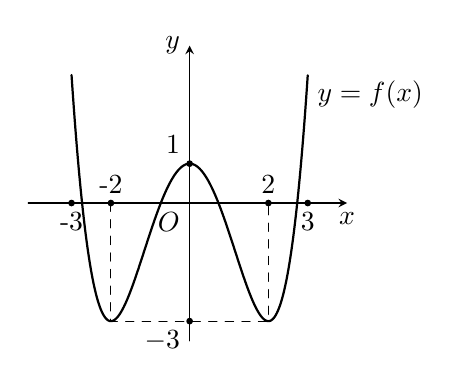
\begin{tikzpicture}[>=stealth,scale=0.5, line join=round, line cap=round]
            \def\f[#1]{0.25*((#1)^4-8*(#1)^2+4)}
            \draw[->] (-4.1,0)--(4,0) node [below]{$x$};
            \draw[->] (0,-3.5)--(0,4) node [left]{$y$};
            \node at (0,0) [below left]{$O$};
            % \clip;
            \draw[domain=-3:3,samples=300,thick] plot (\x,{\f[\x]});
            \foreach \x in {-2,2} \filldraw (\x,0) node[above]{\x} circle (2pt);
            \foreach \x in {-3,3} \filldraw (\x,0) node[below]{\x} circle (2pt);
            \filldraw (0,1) node[above left]{$1$} circle (2pt);
            \filldraw (0,-3) node[below left]{$-3$} circle (2pt);
            \draw[dashed](-2,0)--(-2,-3)--(2,-3)--(2,0);
            \draw (3,2.75) node[right]{$y=f(x)$};
    \end{tikzpicture}}
    \loigiai{%GV tổng quát hóa bài toán:
        Cho hàm số $f(x)$ có đồ thị $(C)$ cho trước. Xác định số đường tiệm cận đứng của đồ thị hàm số $y=\dfrac{u(x)}{v[f(x)]}$.
        \begin{enumerate}
            \item Tìm tập xác định của hàm số $y=\dfrac{u(x)}{v[f(x)]}$.\\
            \item Tìm nghiệm của phương trình $u(x)=0\quad (1)$.\\
            \item Tìm nghiệm của phương trình $v[f(x)]=0\quad (2)$. Giả sử $f(x)=m_1$, $f(x)=m_2,\ldots$.
        \end{enumerate}
        Dựa vào đồ thị $(C)$, xác định hoành độ giao điểm của $(C)$ với các đường thẳng $d_1\colon f(x)=m_1$, $d_2\colon f(x)=m_2,\ldots$.\\
        Số đường tiệm cận đứng của đồ thị hàm số $y=\dfrac{u(x)}{v[f(x)]}$ chính là tổng của:
        \begin{itemize}
            \item Số nghiệm riêng của phương trình $(2)$.
            \item Số nghiệm chung $x=x_0$ của $(1) $ và $(2)$ mà bậc của $(x-x_0)$ ở mẫu lớn hơn bậc của $(x-x_0)$ ở tử.
        \end{itemize}
        \noindent
        Xét hàm số $y=g(x)=\dfrac{(x^2-4)(x^2+2x)}{[f(x)]^2+2f(x)-3}$.
        \immini
        {
            Giải phương trình $(x^2-4)(x^2+2x)=0\,(1)$\\$ \Leftrightarrow \hoac{& x^2-4=0 \\ & x^2+2x=0}\Leftrightarrow \hoac{& x=\pm 2 \\ & x=0.}$\\
            Giải phương trình $[f(x)]^2+2f(x)-3=0\,(2)$\\
            $ \Leftrightarrow \hoac{& f(x)=1 \\ & f(x)=-3.}$\\
        }
        {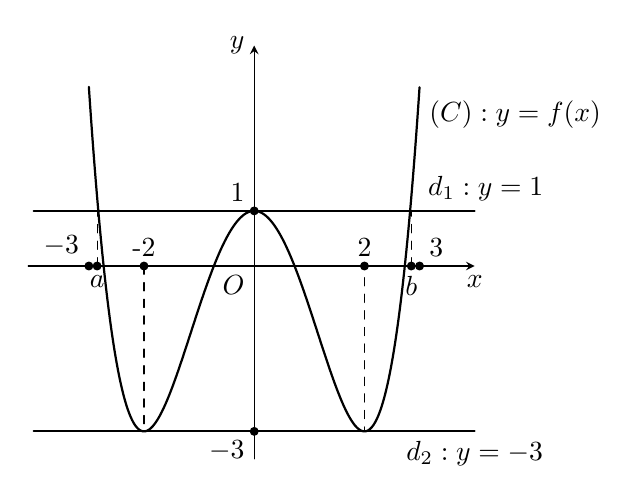
\begin{tikzpicture}[>=stealth,scale=0.7, line join=round, line cap=round]
                \def\f[#1]{0.25*((#1)^4-8*(#1)^2+4)}
                \def\g[#1]{1}
                \def\h[#1]{-3}
                \draw[->] (-4.1,0)--(4,0) node [below]{$x$};
                \draw[->] (0,-3.5)--(0,4) node [left]{$y$};
                \node at (0,0) [below left]{$O$};
                % \clip;
                \draw[domain=-3:3,samples=300,thick] plot (\x,{\f[\x]});
                \draw[domain=-4:4,samples=300,thick] plot (\x,{\g[\x]});
                \draw[domain=-4:4,samples=300,thick] plot (\x,{\h[\x]});
                \foreach \x in {-2,2} \filldraw (\x,0) node[above]{\x} circle (2pt);
                \filldraw (-3,0) node[above left]{$-3$} circle (2pt);
                \filldraw (3,0) node[above right]{$3$} circle (2pt);
                \filldraw (-2.85,0) node[below]{$a$} circle (2pt);
                \filldraw (2.85,0) node[below]{$b$} circle (2pt);
                \filldraw (0,1) node[above left]{$1$} circle (2pt);
                \filldraw (0,-3) node[below left]{$-3$} circle (2pt);
                \draw[dashed](-2,0)--(-2,-3)--(2,-3)--(2,0) (-2.85,0)--(-2.85,1) (2.85,0)--(2.85,1);
                \draw (3,2.75) node[right]{$(C):y=f(x)$};
                \draw (4.2,1) node[above]{$d_1:y=1$};
                \draw (4,-3) node[below]{$d_2:y=-3$};
            \end{tikzpicture}
        }
        Dựa vào đồ thị đã cho $(2)\Leftrightarrow \hoac{& x = \pm 2 \\ & x=0\\&x=a\\&x=b.}$
        với $-3<a<-2<2<b<3$.\\
        Trong điều kiện xác định của hàm số $y=g(x)$ ta có thể viết $$y=g(x)=\dfrac{x(x-2)(x+2)^2}{x^2(x-a)(x-b)(x-2)^2(x+2)^2}=\dfrac{1}{x(x-a)(x-b)(x-2)}$$
        Vậy số tiệm cận đứng của đồ thị hàm số $y=g(x)$ bằng $4$.
    }
\end{ex}
\begin{ex}
    \immini{%Câu 97.
        Đường cong ở hình bên là đồ thị của hàm số $y = ax^3 +bx^2 +cx+d$. Đồ thị hàm số $y =\dfrac{(x+1)\sqrt{1-x}}{f(x^2)}$ có tất cả bao nhiêu tiệm cận đứng?
        \shortans{$2$}
        % \choice
        % {1}
        % {6}
        % {4}
        % {\True 2}
    }{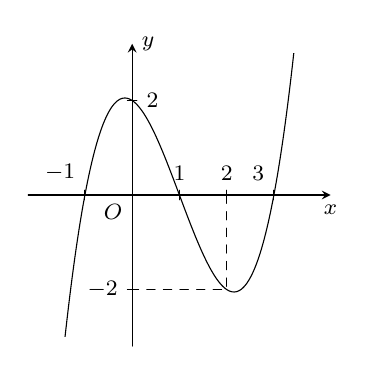
\begin{tikzpicture}[scale=.6, font=\footnotesize, line join=round, line cap=round, >=stealth]
            \def\xmin{-2}\def\xmax{4}\def\ymin{-3}\def\ymax{3}
            \draw[->] (\xmin-0.2,0)--(\xmax+0.2,0) node[below] {\footnotesize $x$};
            \draw[->] (0,\ymin-0.2)--(0,\ymax+0.2) node[right] {\footnotesize $y$};
            \draw (0,0) node [below left] {\footnotesize $O$};
            \foreach \x in {1,2}\draw (\x,-0.1)--(\x,0.1) node [above ] {\footnotesize $\x$};
            \foreach \x in {-1,3}\draw (\x,-0.1)--(\x,0.1) node [above left] {\footnotesize $\x$};
            \foreach \y in {-2}\draw (0.1,\y)--(-0.1,\y) node [left] {\footnotesize $\y$};
            \foreach \y in {2}\draw (-0.1,\y)--(0.1,\y) node [right] {\footnotesize $\y$};
            \clip (\xmin,\ymin) rectangle (\xmax,\ymax);
            \draw[smooth,samples=200,domain=\xmin:\xmax] plot (\x,{0.6666666666666666*((\x)^3)+-2*((\x)^2)+-0.6666666666666666*(\x)+2});
            \draw[dashed] (1.0,0)--(1.0,0.0)--(0,0.0);\fill (1.0,0.0) circle (1pt);
            \draw[dashed] (2,0)--(2,-2)--(0,-2);
    \end{tikzpicture}}
    \loigiai{
        * Điều kiện: $\heva{&f(x^2) \ne 0\\&x \le 1.}$\\
        Nhìn hình vẽ ta thấy
        $f(x^2)=0\Leftrightarrow \hoac{&x^2=-1\\&x^2=1\\&x^2=3}\Leftrightarrow \hoac{&x=\pm 1\,(\text{nghiệm đơn})\\&x=- \sqrt{3}\,(\text{nghiệm đơn})\\&x= \sqrt{3}\,(\text{không thỏa mãn})}.$\\
        Vậy $y=\dfrac{(x+1)\sqrt{1-x}}{f(x^2)}=\dfrac{(x+1)\sqrt{1-x}}{(x - 1)(x + 1)(x + \sqrt{3})}$ \\
        Đồ thị hàm số có 2 đường tiệm cận đứng.}
\end{ex}
\begin{ex}
    \immini{ %Câu 95.
        Đường cong ở hình bên là đồ thị của hàm số $y = ax^3 +bx^2 +cx+d$. Đồ thị hàm số $y =\dfrac{(2x+1)\sqrt{x-1}}{f(|x|)}$ có tất cả bao nhiêu tiệm cận đứng?
        \shortans{$1$}
        % \choice
        % {\True 1}
        % {3}
        % {4}
        % {2}
    }{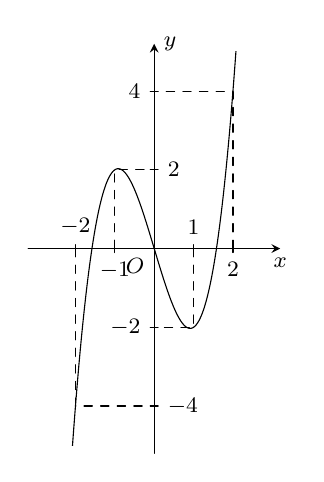
\begin{tikzpicture}[scale=.5, font=\footnotesize, line join=round, line cap=round, >=stealth]
            \def\xmin{-3}\def\xmax{3}\def\ymin{-5}\def\ymax{5}
            \draw[->] (\xmin-0.2,0)--(\xmax+0.2,0) node[below] {\footnotesize $x$};
            \draw[->] (0,\ymin-0.2)--(0,\ymax+0.2) node[right] {\footnotesize $y$};
            \draw (0,0) node [below left] {\footnotesize $O$};
            \foreach \x in {-1,2}\draw (\x,0.1)--(\x,-0.1) node [below] {\footnotesize $\x$};
            \foreach \x in {-2,1}\draw (\x,-0.1)--(\x,0.1) node [above] {\footnotesize $\x$};
            \foreach \y in {-4,2}\draw (-0.1,\y)--(0.1,\y) node [right] {\footnotesize $\y$};
            \foreach \y in {-2,4}\draw (0.1,\y)--(-0.1,\y) node [left] {\footnotesize $\y$};
            \clip (\xmin,\ymin) rectangle (\xmax,\ymax);
            \draw[smooth,samples=200,domain=\xmin:\xmax] plot (\x,{1.3333333333333333*((\x)^3)+0*((\x)^2)+-3.3333333333333335*(\x)+0});
            \draw[dashed] (-2,0)--(-2,-4)--(0,-4);
            \draw[dashed] (2,0)--(2,4)--(0,4);
            \draw[dashed] (1,0)--(1,-2)--(0,-2);
            \draw[dashed] (-1,0)--(-1,2)--(0,2);
    \end{tikzpicture}}
    \loigiai{
        * Điều kiện: $\heva{&f(|x|) \ne 0\\&x \ge 1.}$\\
        Nhìn hình vẽ ta thấy
        $f(|x|)=0\Leftrightarrow \hoac{&|x|=x_1\,(-2<x_1<-1)\\&|x|=0\\&|x|=x_2\,(1<x_2<2)}\Leftrightarrow \hoac{&x=0&(\text{không thỏa mãn})\\&x=- x_2&(\text{không thỏa mãn})\\&x=x_2&(\text{nghiệm đơn}).}$\\
        Vậy $y =\dfrac{(2x+1)\sqrt{x-1}}{f(|x|)}=\dfrac{(2x+1)\sqrt{x-1}}{ax(x+x_2)(x-x_2)}.$ \\
        Đồ thị hàm số có 1 đường tiệm cận đứng.}
\end{ex}
\begin{ex}
    Đáp ứng tần số của một hệ thống điều khiển có thể được mô tả bởi hàm truyền \( H(s) = \dfrac{\omega_n^2}{s^2 + 2\zeta\omega_ns + \omega_n^2} \), trong đó \( \omega_n \) là tần số tự nhiên và \( \zeta \) là hệ số tắt dần. Tìm đường tiệm cận ngang của đáp ứng tần số khi tần số góc \( s \) tăng và nêu ý nghĩa của nó.
    \shortans{$y=0$}
    \loigiai{
        Khi \( s \) tăng vô hạn, các thành phần bậc cao trong mẫu số chiếm ưu thế:
        \[
        H(s) \approx \frac{\omega_n^2}{s^2}
        \]
        Đường tiệm cận ngang của \( H(s) \) khi \( s \to \infty \) là:
        \[
        |H(s)| \approx \frac{\omega_n^2}{s^2} \to 0
        \]}
\end{ex}
\begin{ex}
    Trong thuyết tương đối của Einstein, khối lượng của vật chuyển động với vận tốc $v$ được cho bởi công thức:
    $$m(v)=\dfrac{m_0}{\sqrt{1-\dfrac{v^2}{c^2}}},$$
    trong đó $m_0$ là khối lượng của vật khi nó đứng yên, $c$ là vận tốc ánh sáng.\\
    (nguồn: https://www.britannica.com/science/relativity/Relativistic-mass)\\
    Xem $m$ là hàm số theo vận tốc $v$, tìm đường tiệm cận đứng của đồ thị hàm số. Từ đó nhận xét khối lượng của vật khi vận tốc của nó càng gần với vận tốc ánh sáng.
    \shortans{$v=c$, khối lượng tăng lên vô hạn}
    \loigiai{
        Điều kiện xác định: $\heva{&1-\dfrac{v^2}{c^2}>0\\
            &v>0}\Leftrightarrow\heva{& -c<v<c\\
            &v>0}\Leftrightarrow 0<v<c$.\\
        Ta có $\lim\limits_{v\to c^{-}} m(v)=\lim\limits_{v\to c^{-}}\dfrac{m_0}{\sqrt{1-\dfrac{v^2}{c^2}}}=+\infty$ nên đường thẳng $v=c$ là tiệm cận đứng của đồ thị hàm số.\\
        Từ đó ta suy ra khi vận tốc của vật càng sát với vận tốc ánh sáng thì khối lượng của vật tăng lên vô hạn.
    }
\end{ex}
\Closesolutionfile{ans}